\documentclass{article}

\usepackage[T1]{fontenc}
\usepackage[utf8]{inputenc}
\usepackage[brazilian]{babel}
\usepackage{graphicx}
\usepackage[export]{adjustbox}[2011/08/13]
\usepackage{float}
\usepackage[pdftex]{hyperref}
\usepackage{epstopdf}
\usepackage{etoolbox}
\usepackage{amsmath}
\usepackage{amsfonts}
\usepackage{amssymb}
\usepackage{caption}
\usepackage{subcaption}
\usepackage{setspace}
\usepackage{tikz}
\usepackage{listings}
\usepackage{xcolor} 

\bibliographystyle{eric}
\patchcmd{\thebibliography}{\section*}{\section}{}{}


\newcommand{\R}{\ensuremath{\mathbb{R}}}
\newcommand{\Prob}{\ensuremath{\mathbb{P}}}
\newcommand{\K}{\ensuremath{\mathbb{K}}}
\newcommand{\U}{\ensuremath{\mathbb{U}}}
\newcommand{\N}{\ensuremath{\mathbb{N}}}
\newcommand{\Lg}{\ensuremath{\mathbb{L}}}
\newcommand{\T}{\ensuremath{\rm Tr}}
\newcommand{\sg}{{\sigma(x_k)}}

\newcommand{\G}{\ensuremath{\mathcal{G}}}
\newcommand{\F}{\ensuremath{\mathcal{F}}}
\newcommand{\C}{\ensuremath{\mathcal{C}}}
\newcommand{\E}{\ensuremath{\mathcal{E}}}
\newcommand{\Hn}{\ensuremath{\mathcal{H}}}
\newcommand{\Hoo}{\ensuremath{\mathcal{H}_\infty}}
\newcommand{\Hop}{\ensuremath{\mathcal{H}_{op}}}
% --------------------------------------------------
\newtheorem{theo}{Teorema}
\newtheorem{exa}{Exemplo}
\newtheorem{lemm}{Lema}
\newtheorem{coro}{Corolário}
\newtheorem{defn}{Definição}[section]

\begin{document}

\begin{titlepage}
\begin{center}

\newcommand{\HRule}{\rule{\linewidth}{0.5mm}}
% Upper part of the page. The '~' is needed because \\
% only works if a paragraph has started.

\includegraphics[width=0.15\textwidth]{logoUnicamp}~\\[1cm]

\textsc{\LARGE Universidade Estadual de Campinas}\\[1.5cm]

\textsc{\Large Faculdade de Engenharia Mecânica}\\[0.5cm]

% Title
\HRule \\[0.4cm]
{ \huge \bfseries ES664 - Laboratório de Eletrônica para Automação Industrial\\ \vspace{1cm} Relatório - Experimento 4\\
\Large{Acionamento de motor DC} \\[0.4cm] }

\HRule \\[1.5cm]

% Author and supervisor
\begin{minipage}{0.6\textwidth}
\begin{flushleft} \large
\emph{Nome:}\\
Daniel Dello Russo Oliveira\\Marcelli Tiemi Kian
\end{flushleft}
\end{minipage}
\begin{minipage}{0.2\textwidth}
\begin{flushright} \large
\emph{RA}\\ 101918\\117892
\end{flushright}
\end{minipage}

\vfill

% Bottom of the page
{\large \today}

\end{center}
\end{titlepage}


\onehalfspacing
\section{Objetivos}
	Este projeto tem como objetivo realizar o acionamento de um motor DC utilizando conversor de potência, controlar a posição por meio de servo-acionamento, e integrar componentes elétricos e mecânicos por malha de controle. 

\section{Motor e Conversor de Potência}
Implementamos no Simulink o circuito apresentado na figura \ref{fig:sim1}. Configuramos o bloco do motor DC disponível para que atuasse como motor DC de ímãs permanentes. Definimos os parâmetros do motor conforme especificado na tabela \ref{tab:param}.

\begin{figure}[H]
	\centering
	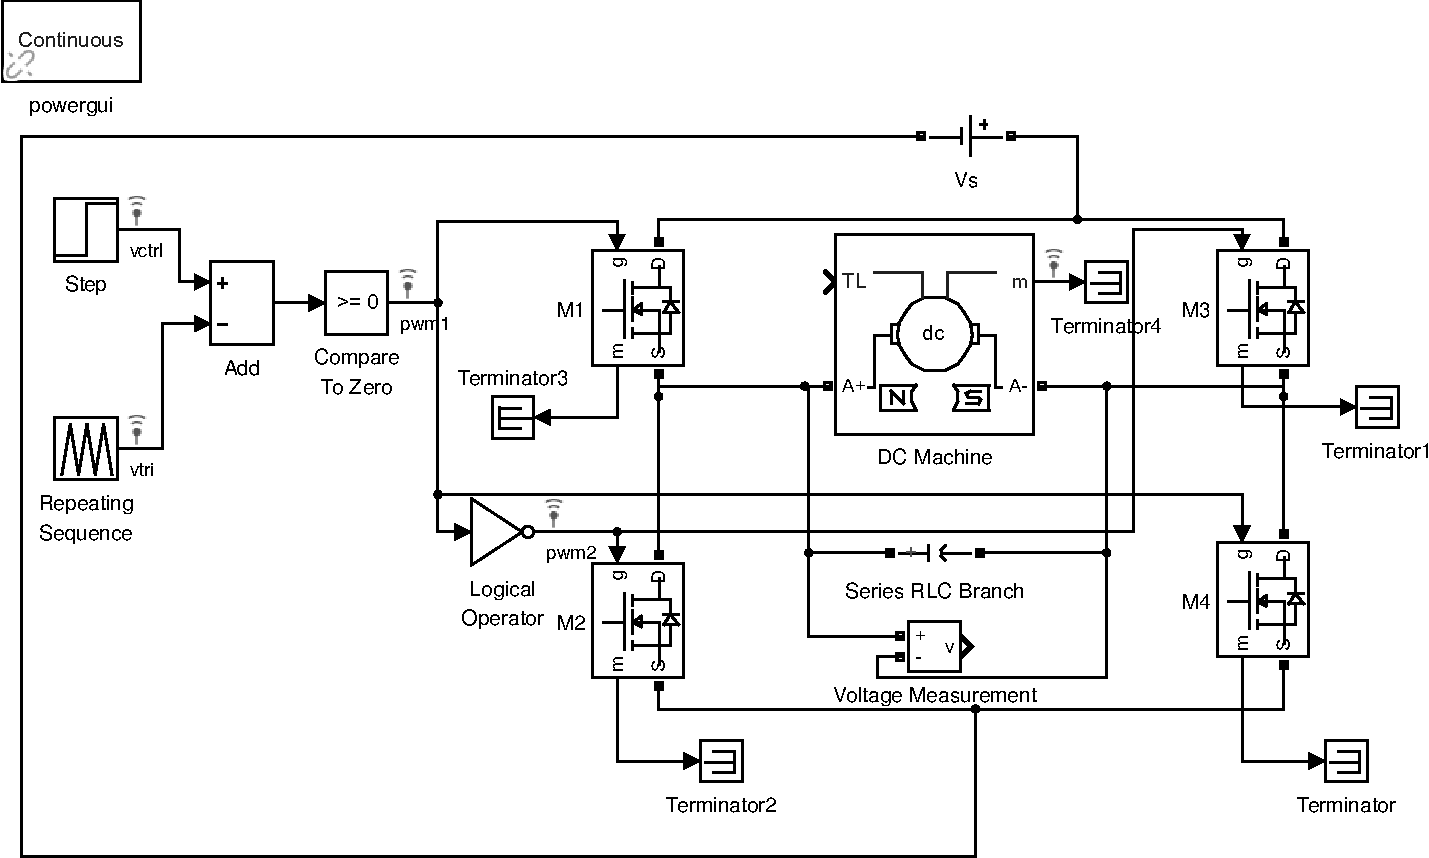
\includegraphics[width=\linewidth]{matlab/sim1}
	\caption{Esquemático da simulação para dimensionamento do motor DC e conversor}
	\label{fig:sim1}
\end{figure}

\begin{table}[]
	\centering
	\caption{Parâmetros do motor DC}
	\label{tab:param}
	\begin{tabular}{|c|c|}
		\hline
		\textbf{Parâmetro}              & \textbf{Valor}                 \\ \hline
		Potência nominal                & $5\ HP$                        \\ \hline
		Velocidade nominal              & $1750\ rpm$                    \\ \hline
		Tensão nominal                  & $240\ V$                       \\ \hline
		Resistência de armadura ($R_a$) & $2,58\ \Omega$                 \\ \hline
		Indutância de armadura ($L_a$)  & $28\ mH$                       \\ \hline
		Inércia ($J$)                   & $2,22 \times 10^{-2}\ kg\ m^2$ \\ \hline
		Atrito viscoso ($B$)            & $2,95 \times 10^{-3}\ N\ m\ s$ \\ \hline
	\end{tabular}
\end{table}

Para o acionamento do motor, utilizamos uma ponte H composta por MOSFETs, sendo que o circuito de acionamento funciona com a diferença de potencial entre sinal de controle ($v_{cont}$) e uma onda triangular ($v_{tri}$), com funcionamento explicado pela figura \ref{fig:ponte}. Para fins de simulação utilizamos $v_{cont}$ e $v_{tri}$ variando entre $0\ V$ e $100\ V$, mas este valor pode variar desde que atenda aos requisitos de acionamento do MOSFET.

\begin{figure}[H]
	\centering
	\begin{subfigure}[t]{0.45\textwidth}
		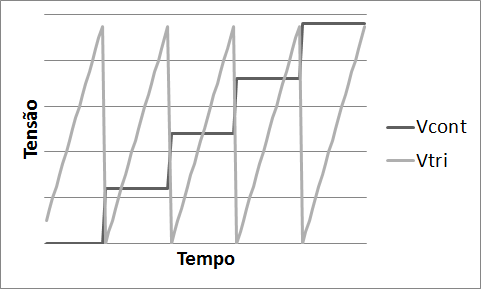
\includegraphics[width=\linewidth]{ponte1}
		\caption{Controle e onda triangular}
	\end{subfigure}
	\begin{subfigure}[t]{0.45\textwidth}
		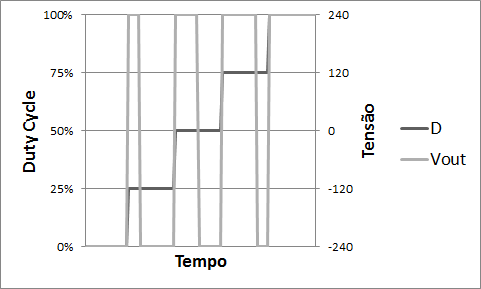
\includegraphics[width=\linewidth]{ponte2}
		\caption{Duty cycle e tensão de saída}
	\end{subfigure}
	\caption{Esquema de funcionamento do circuito de controle da ponte H}	
	\label{fig:ponte}
\end{figure}

A fim de garantir um bom fator de forma na saída do conversor, colocamos um capacitor de filtro $C_f$ em paralelo com a carga. Para o motor em questão chegamos ao seguinte valor:

\begin{equation}
C_f=1000\ \mu F
\end{equation}

Fizemos a simulação da resposta do motor a um degrau com $V_{out}=240\ V$, sem cargas, apenas com os parâmetros físicos definidos nele mesmo.
Obtivemos os resultados de tensão e correntes de armadura ($v_a$ e $i_a$), e também curvas de torque e velocidade angular ($T_{em}$ e $\omega_m$) conforme figura \ref{fig:sim1viwt}.

%TODO: comentar sobre resposta ao degrau

\begin{figure}[h]
	\centering
	\begin{subfigure}{0.45\textwidth}
		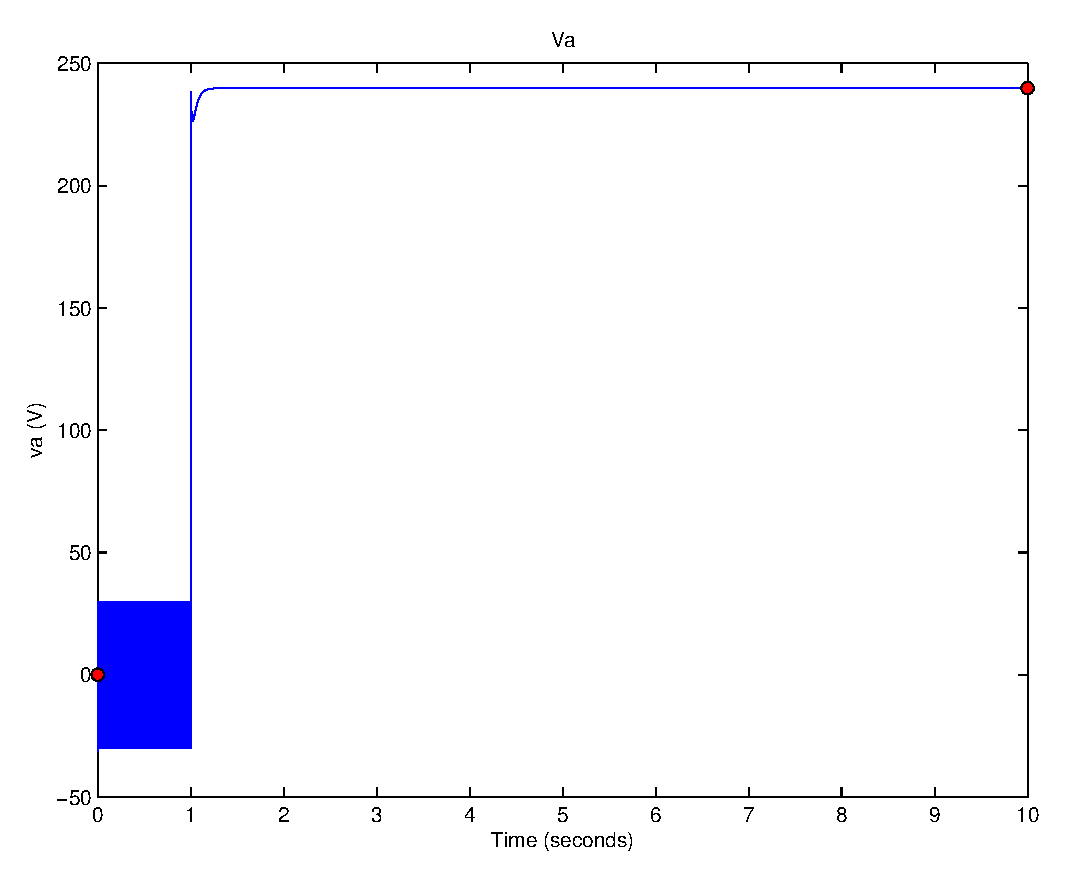
\includegraphics[width=\linewidth]{matlab/va1}
		\caption{Tensão de armadura}
	\end{subfigure}
	\begin{subfigure}{0.45\textwidth}
		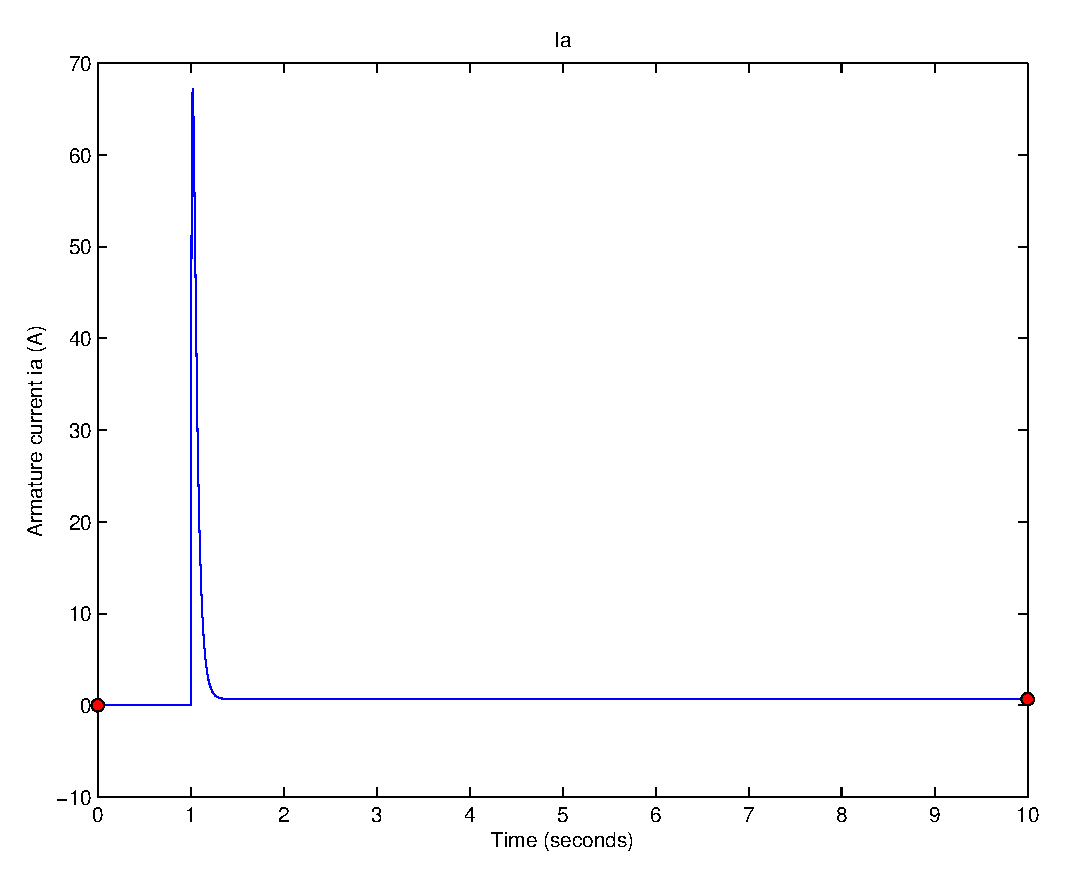
\includegraphics[width=\linewidth]{matlab/ia1}
		\caption{Corrente de armadura}
	\end{subfigure}
	\begin{subfigure}{0.45\textwidth}
		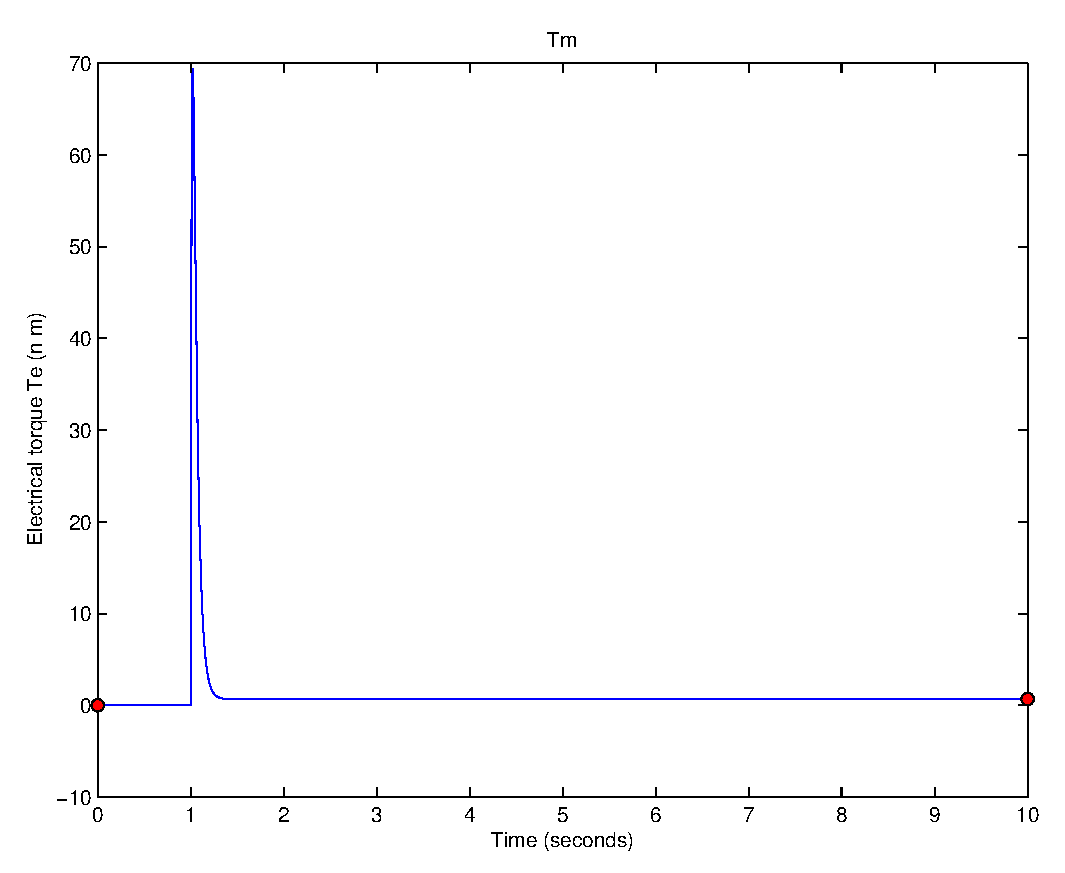
\includegraphics[width=\linewidth]{matlab/tm1}
		\caption{Torque}
	\end{subfigure}
	\begin{subfigure}{0.45\textwidth}
		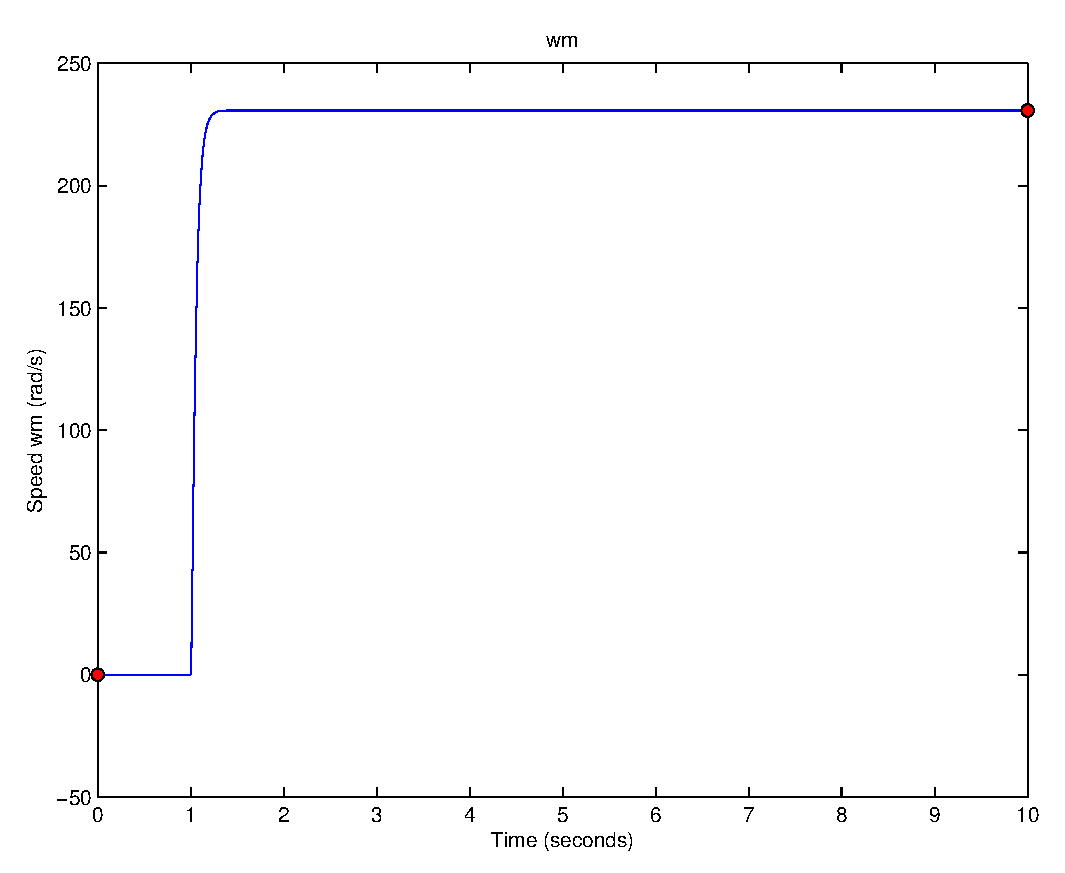
\includegraphics[width=\linewidth]{matlab/wm1}
		\caption{Velocidade angular}
	\end{subfigure}
	\caption{Resposta ao degrau de $240\ V$ no motor DC}	
	\label{fig:sim1viwt}
\end{figure}

\section{Servo-acionamento}
Iniciamos o projeto do servo-acionamento pelo controle PI de corrente. Utilizando o Simulink, conforme figura \ref{fig:sim2}.

\begin{figure}[H]
	\centering
	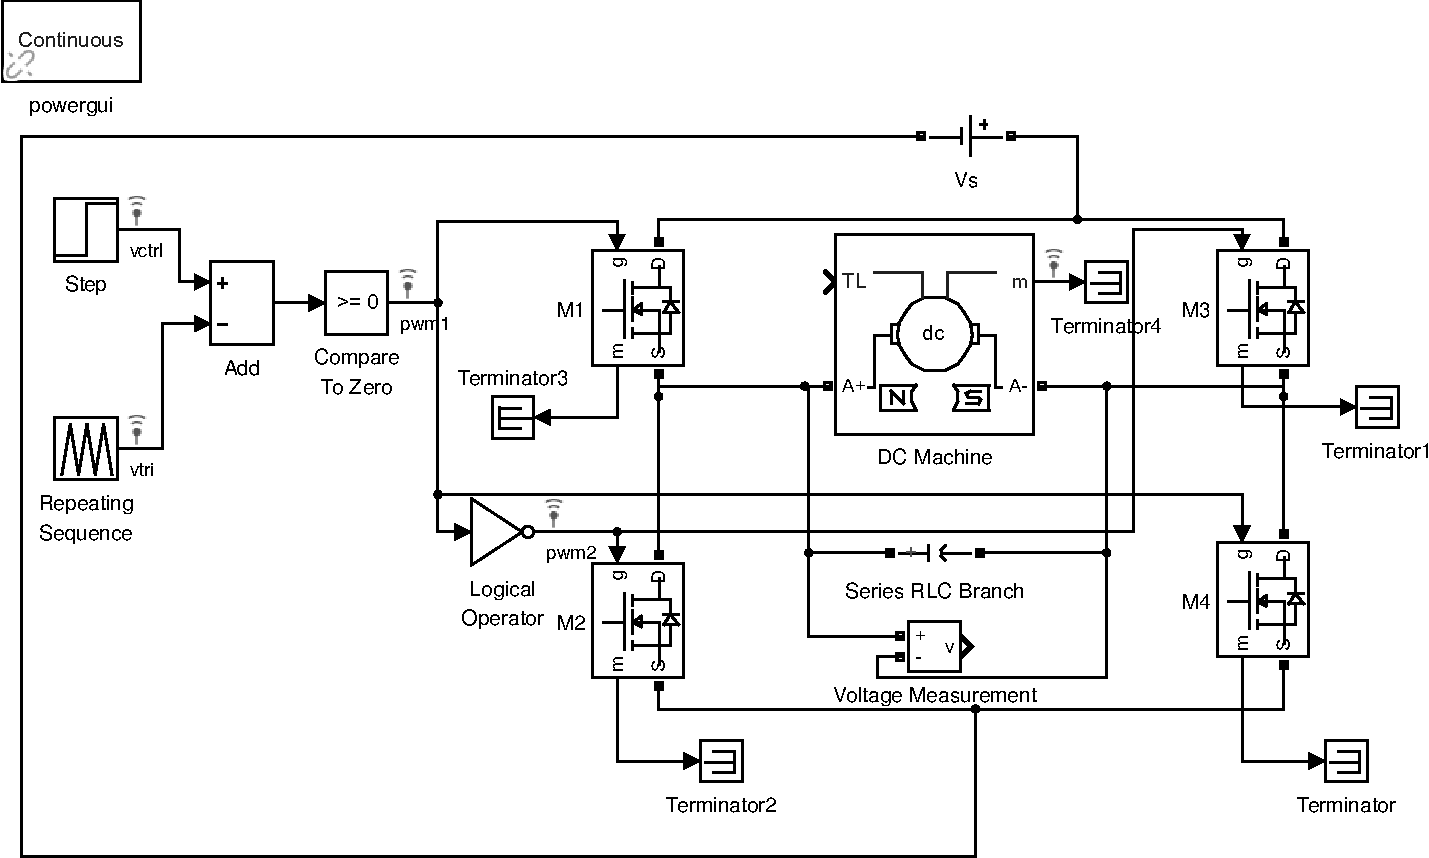
\includegraphics[width=\linewidth]{matlab/sim1}
	\caption{Esquemático da simulação do controlador de corrente}
	\label{fig:sim2}
\end{figure}

\section{Modelagem do Manipulador}
\section{Acoplamento Motor-Robô}


\bibliography{mybib}
\end{document}

